
\chapter{PENDAHULUAN}

\section{Latar Belakang}
% Tentang Citra digital
Citra digital merupakan citra yang dihasilkan dari pengolahan secara digital dengan merepresentasikan citra secara numerik dengan nilai-nilai diskret. Suatu citra digital dapat direpresentasikan dalam bentuk matriks dengan fungsi f(x,y) yang terdiri dari M kolom dan N baris. Perpotongan antara baris dan kolom disebut pixel. Setiap pixel mewakili sebuah warna, pada citra biner sebuah pixel hanya berwarna hitam atau putih saja, pada citra grayscale warna sebuah pixel mewakili tingkat keabuannya (\cite{book:darma}).

% Stream Video adalah
Video stream dapat dipandang sebagai serangkaian citra digital berturut-turut. (\cite{thesis:jin})
% Deteksi Tepi dan Algoritmanya
% 
% FPGA sebagai alat untuk implementasi
% Masalah Performa dan komputasi

\section{Rumusan Masalah}
\blindtext

\section{Batasan Masalah}
\blindtext

\section{Tujuan Penelitian}
\blindtext

\section{Manfaat Penelitian}
\blindtext




\begin{afigure}{Sebuah gambar}
    \label{fig:figure2}
    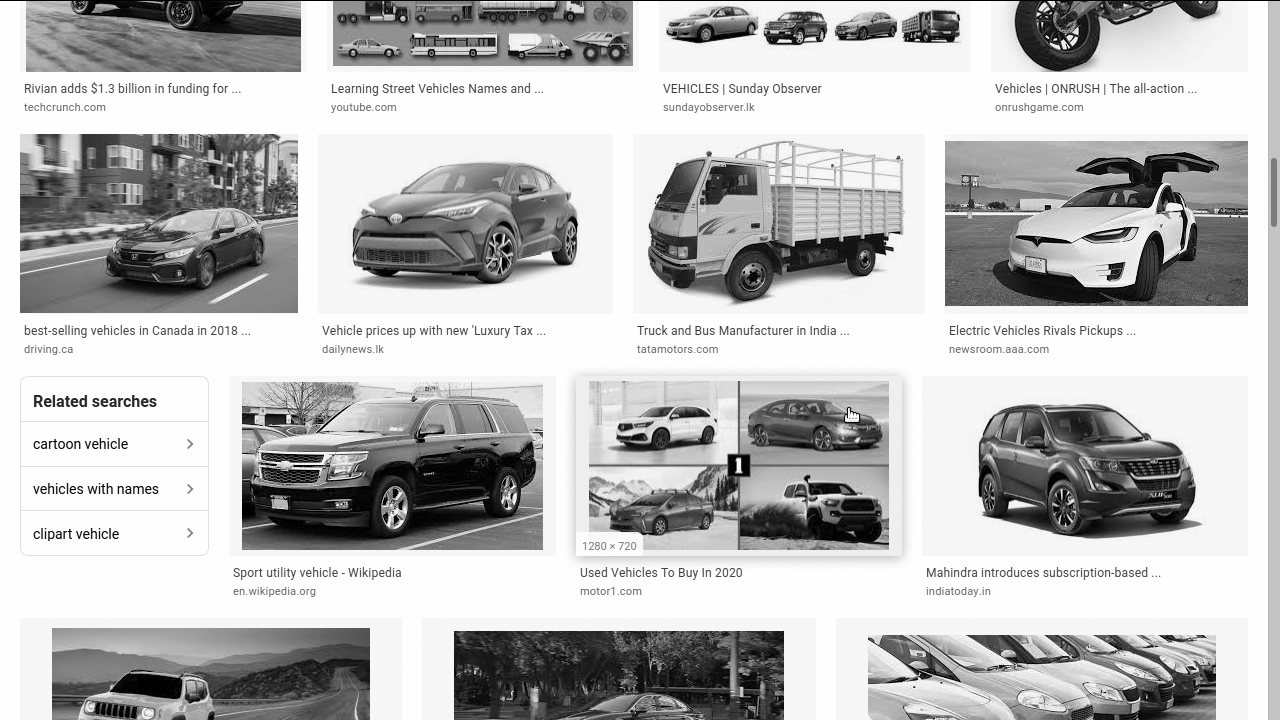
\includegraphics[width=0.5\textwidth, center]{images/input.png}
\end{afigure}

\begin{atable}{Ini Caption tabel}
    \label{table:tabl}
    \begin{tabular}{|l|l|l|l|l|}
    \hline
    fad  & dfaf & fdsfdfads & fdasf & fda  \\
    \hline
    fdas & fdas & ss        & ss    & ss   \\
    \hline
    ss   & dfa  & dfsa      & fdsa  & fdsa \\
    \hline
    ddd  & fdd  & dda       & da    & da \\
    \hline
    \end{tabular}
\end{atable}

\blindtext
~\ref{fig:figure2}
\\
for reference ~\ref{table:tabl}

\begin{afigure}{ini gambar na}
    \label{fig:f1}
    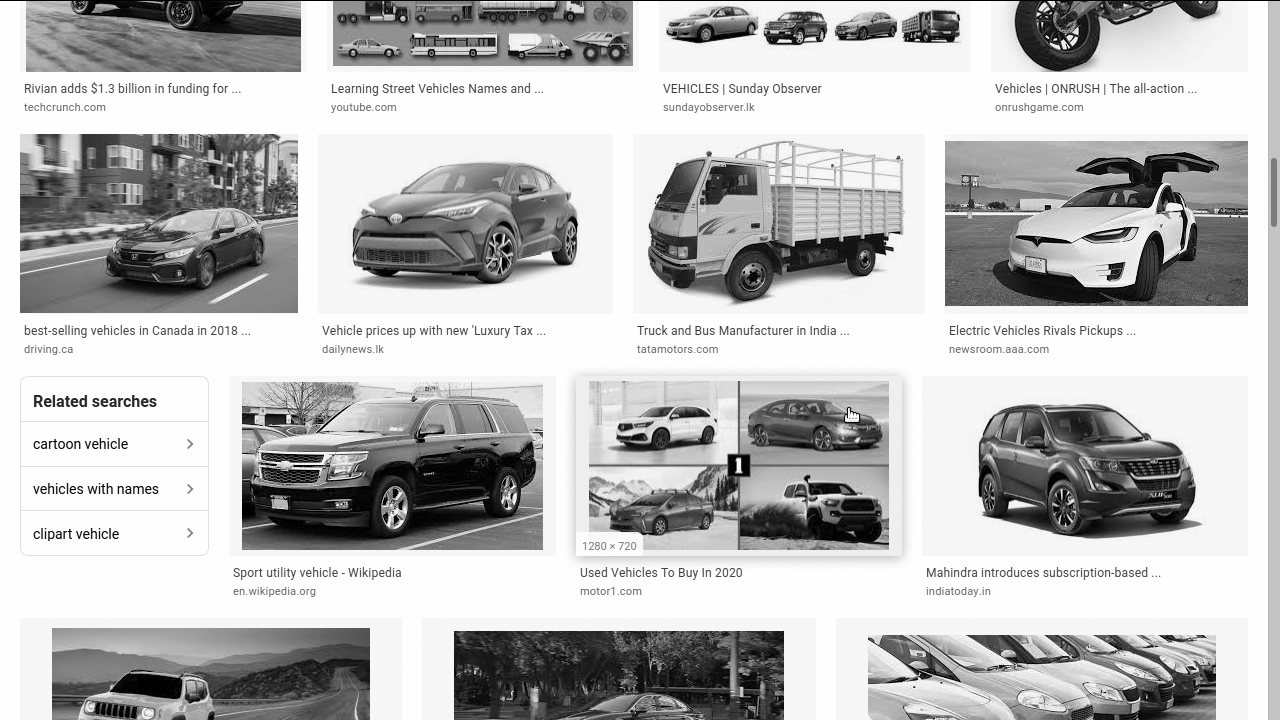
\includegraphics[width=0.5\textwidth, center]{images/input.png}
\end{afigure}
